\pagestyle{plain}
\chapter{Introduction}





\section{Énoncé du problème}
Le suivi d'objet par vision par ordinateur a toujours été, et est encore, un problème suscitant beaucoup d'intérêt et qui fait l'objet de beaucoup de sujets de recherche.\\
En effet, le suivi d'objet apparait dans plein de domaines, comme par exemple:
\begin{itemize}
	\item L'aérospatial, avec l'arrimage de modules à l'ISS, ou encore le suivi de débris spatiaux pour ensuite les faire sortir d'orbites sensibles.
	\item Le militaire, avec le suivi de missiles pour interception précise.
	\item L'astrophysique, avec le suivi de corps célestes.
	\item L'étude de populations animales, comme l'étude de cycles migratoires ou du comportement de certaines espèces.\\
\end{itemize}

Le projet se place dans le contexte du suivi de seiches en milieu aquatique grâce à des vidéos.\\
Les vidéos sous-marines sont sujettes à beaucoup de difficultés, comme la variation de couleur, de lumière et de contraste d'une image à l'autre, la dégradation de la qualité de la vidéo par des sédiments, les mouvements instables du plongeur, ou encore l'arrière plan qui change.\\
Les solutions implémentées doivent essayer de prendre en compte toutes ces variations ainsi que la forme générale de la seiche au cours de ses mouvements (voir figure \ref{fig:cuttlefish_variation}).\\
Le projet a pour objectif de fournir un outil qui propose des solutions qui répondent à toutes ces contraintes, pour suivre des seiches de façon non intrusive (pas de capteurs sur la seiche suivie), afin de limiter l'interaction humaine avec les seiches.

\begin{figure}[!htbp]
\center
	\subfloat{{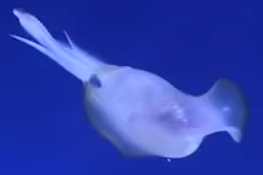
\includegraphics[height=3cm]{cuttlefish_variation1.png}}}
	\hspace{0.5cm}
	\subfloat{{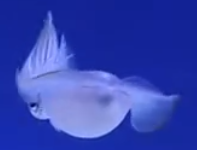
\includegraphics[height=3cm]{cuttlefish_variation2.png}}}
	\\
	\subfloat{{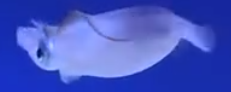
\includegraphics[height=3cm]{cuttlefish_variation3.png}}}
	\hspace{0.5cm}
	\subfloat{{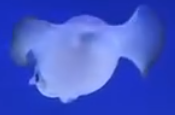
\includegraphics[height=3cm]{cuttlefish_variation4.png}}}
\caption{Différentes apparences d'une même seiche dans une vidéo.}
\label{fig:cuttlefish_variation}
\end{figure}
\FloatBarrier
\clearpage





\section{Motivation}
Le suivi d'objet, de manière générale, étant un problème que l'on rencontre dans beaucoup de domaines liés à l'informatique, les précédents exemples n'étant qu'un petit aperçu, c'est donc un problème de choix à étudier lors de notre parcours d'études.\\
De plus, il permet d'introduire des concepts et des algorithmes fondamentaux, comme le concept de filtrage de signaux, ou d'espace de représentation, ou encore, les algorithmes de filtrage, de descripteurs, ou de mesures de similarité.\\
Ces concepts et algorithmes sont récurrents dans le monde de l'informatique et plus précisément quand il s'agit de faire du traitement du signal ou de la vision par ordinateur.\\
Se familiariser dès à présent avec ces différentes notions pourra grandement nous aider dans la suite de notre parcours.\\




\section{Méthodes}
Il existe beaucoup d'approches possibles pour résoudre le problème de suivi d'objet, approches parmi lesquelles ont peut noter:\\
\begin{itemize}
	\item \textit{Intelligence Artificielle}\newline
	Cette approche est de plus en plus populaire, notamment avec des modèles comme YOLO\cite{redmon_you_2016} ou SSD\cite{liu_ssd_2016}. Ces modèles peuvent directement donner la bounding box de l'objet suivi, sans avoir à faire de traitement sur la sortie du modèle.\\
	Cependant, cette approche est peu résistante à l'occlusion de l'objet suivi.\\
	
	\item \textit{Capteurs}\newline
	Cette approche utilise, par exemple, des IMUs ou marqueurs infrarouges, qui peuvent donner des informations sur l'accélération linéaire ou angulaire. Ces informations sont ensuite filtrées grâce à des algorithmes de filtrage, comme le filtre de Kalman (linéaire ou non), ou encore le filtre à particule.\\
	Cependant, cette approche nécessite de poser des capteurs sur l'objet à suivre.\\
	
	\item \textit{Photogrammétrie}\newline
	Cette approche utilise des descripteurs d'image pour extraire des features importantes et ensuite, matcher ces features avec d'autres images pour pouvoir estimer le déplacement de la caméra.\\
	Cependant, cette approche est plus utilisée dans le cas ou l'on cherche à savoir où est-ce que le caméraman se situe, plutôt qu'un objet qui se trouve dans une image (comme le SLAM).\\
	
	\item \textit{Hybride}\newline
	Cette approche combine différentes parties des méthodes déjà présentées et est celle sur laquelle ce projet est basé.\\
	On utilise l'intelligence artificielle pour détecter un objet d'intérêt à suivre dans une séquence d'images, la partie filtrage de l'approche avec des capteurs pour améliorer nos estimations de l'état de l'objet suivi, et enfin, la photogrammétrie pour récupérer les features intéressantes dans une image et les comparer avec les features d'une image de référence.\\
	Cette approche est cependant assez sensible aux paramètres que nous lui donnons, ainsi qu'à certaines caractéristiques des images données en entrée, comme le contraste, la résolution ou encore la colorimétrie.
	Le détail de cette approche sera donné en partie \hyperlink{chapter.3}{3}.\\
\end{itemize}





\section{Cahier des charges}

\subsection{Besoins fonctionnels}
Les besoins peuvent être séparés en 5 catégories:
\begin{enumerate}
	\item Le besoin d'une intelligence artificielle pour effectuer la détection initiale.
	\item Le besoin de descripteurs pour récupérer un vecteur qui décrit une image donnée.
	\item Le besoin de mesures de similarité pour comparer un vecteur caractéristique d'une image avec un descripteur de référence.
	\item Le besoin d'un filtre à particule permettant d'estimer certaines propriétés de la seiche que l'on suit.
	\item Le besoin d'un programme principal permettant d'agencer chacune des parties ensemble.\\
\end{enumerate}

Les différents descripteurs et mesures de similarité devront pouvoir être utilisés par le filtre à particule afin de mettre à jour l'état de chacune des particules. Par extension, le filtre à particule devra être modulable, afin de fonctionner avec ces différents descripteurs et mesures de similarité, ainsi que de répondre aux demandes du programme principal.\\
Le programme principal se charge de l'initialisation des différents modules ainsi que de l'affichage de données clefs (visualisation de  résultats).\\

\subsection{Besoins non-fonctionnels}
Les formats vidéos acceptés sont libres.\\
La résolution des vidéos est également libre, mais une préférence sera portée pour la résolution 640x640 (résolution utilisée pour entrainer l'intelligence artificielle).\\
Le programme doit pouvoir tourner sur Windows, Linux et OSX.\\
Le programme doit pouvoir sauvegarder le résultat obtenu en une vidéo et également sauvegarder les bounding box dans un fichier texte.\\

\subsection{Contraintes}
Aucun budget n'a été alloué pour le projet, le travail s'effectuera sur nos machines personnelles, ou sur les machines mises à disposition par l'université.\\
Le projet doit être complété en 4 mois, avec une vingtaine de jours supplémentaires pour la rédaction du rapport.\\


\clearpage
